\حصہ{قطبی محدد میں ترسیم}
اس حصہ میں مساوات کو قطبی محدد میں ترسیم کرنے کے تراکیب پر غور کیا جائے گا۔

\جزوحصہء{تشاکلی}
قطبی محدد میں تشاکلی کا معیاری پرکھ شکل \حوالہ{شکل_مخروط_تشاکلی_پرکھ_قطبی} میں دکھایا گیا ہے۔
\begin{figure}
\centering
\begin{subfigure}{0.3\textwidth}
\centering
\begin{tikzpicture}
\draw[-latex](-1.5,0)--(1.5,0)node[right]{$x$};
\draw[-latex](0,-1.25)--(0,1.5)node[above]{$y$};
\draw(1,1)node[circ]{}node[right]{$(r,\theta)$}--(0,0)node[below left]{$O$}--(1,-1)node[circ]{}
node[right]{$\begin{aligned}&(r,-\theta)\\ &(-r,\pi-\theta)\, \text{یا}\end{aligned}$}--(1,1);
\end{tikzpicture}
\caption{محور \عددی{x} کے لحاظ سے۔}
\end{subfigure}\hfill
\begin{subfigure}{0.3\textwidth}
\centering
\begin{tikzpicture}
\draw[-latex](-1.5,0)--(1.5,0)node[right]{$x$};
\draw[-latex](0,-1.25)--(0,1.5)node[above]{$y$};
\draw(1,1)node[circ]{}node[above]{$(r,\theta)$}--(0,0)node[below left]{$O$}--(-1,1)node[circ]{}
node[above]{$\begin{aligned} &(r,\pi-\theta)\\ &(-r,-\theta)\, \text{یا}  \end{aligned}$}--(1,1);
\end{tikzpicture}
\caption{محور \عددی{y} کے لحاظ سے۔}
\end{subfigure}\hfill
\begin{subfigure}{0.3\textwidth}
\centering
\begin{tikzpicture}
\draw[-latex](-1.5,0)--(1.5,0)node[right]{$x$};
\draw[-latex](0,-1.25)--(0,1.5)node[above]{$y$};
\draw(1,1)node[circ]{}node[above]{$(r,\theta)$}--(-1,-1)node[circ]{}node[below]{$\begin{aligned}&(-r,\theta)\\  &(r,\theta+\pi)\,\text{یا}\end{aligned}$};
\draw(0,0)node[below left]{$O$};
\end{tikzpicture}
\caption{مبدا کے لحاظ سے۔}
\end{subfigure}
\caption{تشاکلی کے تین پرکھ۔}
\label{شکل_مخروط_تشاکلی_پرکھ_قطبی}
\end{figure}

\موٹا{قطبی ترسیمات کے پرکھ تشاکلی}\\
\begin{enumerate}[a.]
\item
\ترچھا{محور \عددی{x} کے لحاظ سے تشاکلی:} اگر نقطہ \عددی{(r,\theta)} ترسیم پر پایا جاتا ہو تب نقطہ \عددی{(r,-\theta)} یا
 \عددی{(-r,\pi-\theta)} بھی ترسیم پر پایا جائے گا (شکل \حوالہ{شکل_مخروط_تشاکلی_پرکھ_قطبی}-ا)۔
\item
\ترچھا{محور \عددی{y} کے لحاظ سے تشاکلی:}  اگر نقطہ \عددی{(r,\theta)} ترسیم پر پایا جاتا ہو تب نقطہ \عددی{(r,\pi-\theta)} یا 
\عددی{(-r,-\theta)} بھی ترسیم پر پایا جائے گا (شکل \حوالہ{شکل_مخروط_تشاکلی_پرکھ_قطبی}-ب)۔
\item
\ترچھا{مبدا کے لحاظ سے تشاکلی:}  اگر نقطہ \عددی{(r,\theta)} ترسیم پر پایا جاتا ہو تب نقطہ \عددی{(-r,\theta)} یا 
\عددی{(r,\theta+\pi)} بھی ترسیم پر پایا جائے گا (شکل \حوالہ{شکل_مخروط_تشاکلی_پرکھ_قطبی}-ج)۔
\end{enumerate}

\جزوحصہء{ڈھلوان}
قطبی منحنی \عددی{r=f(\theta)} کی ڈھلوان \عددی{\tfrac{\dif y}{\dif x}} ہے نا کہ \عددی{r'=\tfrac{\dif f}{\dif \theta}}۔ اس کی وجہ سمجھنے کی خاطر \عددی{f} کی ترسیم کو درج ذیل مقدار معلوم مساوات کی ترسیم فرض کریں۔
\begin{align*}
x=r\cos\theta=f(\theta)\cos\theta,\quad y=r\sin\theta=f(\theta)\sin\theta
\end{align*}
اگر \عددی{f} متغیر \عددی{\theta} کا قابل تفرق تفاعل ہو تب \عددی{x} اور \عددی{y} بھی \عددی{\theta} کے قابل تفرق تفاعل ہوں گے اور جب \عددی{\tfrac{\dif x}{\dif\theta}\ne 0} ہو تب ہم \عددی{\tfrac{\dif y}{\dif x}}  کو درج ذیل مقدار معلوم کلیہ سے اخذ کر سکتے ہیں۔
\begin{align*}
\frac{\dif y}{\dif x}&=\frac{\dif y/\dif \theta}{\dif x/\dif \theta}&&\text{\RL{مساوات \حوالہ{مساوات_مخروط_زنجیری_قاعدہ_الف}}}\\
&=\frac{\tfrac{\dif}{\dif\theta}(f(\theta)\cdot\sin\theta)}{\tfrac{\dif}{\dif\theta}(f(\theta)\cdot\cos\theta)}\\
&=\frac{\tfrac{\dif f}{\dif \theta}\sin\theta+f(\theta)\cos\theta}{\tfrac{\dif f}{\dif \theta}\cos\theta-f(\theta)\sin\theta}&&\text{\RL{تفرق کا کلیہ ضرب}}
\end{align*}

\موٹا{منحنی \عددی{r=f(\theta)} کی ڈھلوان} جہاں \عددی{(r,\theta)} پر \عددی{\tfrac{\dif x}{\dif\theta}\ne 0} ہونا ضروری ہے۔
\begin{align}\label{مساوات_مخروط_قطبی_ڈھلوان_الف}
\left. \frac{\dif y}{\dif x}\right\vert_{(r,\theta)}=\frac{f'(\theta)\sin\theta+f(\theta)\cos\theta}{f'(\theta)\cos\theta-f(\theta)\sin\theta}&&\tfrac{\dif x}{\dif \theta}\ne 0
\end{align}

اگر مبدا پر منحنی \عددی{r=f(\theta)} کا زاویہ \عددی{\theta=\theta_0} ہو تب \عددی{f(\theta_0)=0} ہو گا اور مساوات \حوالہ{مساوات_مخروط_قطبی_ڈھلوان_الف} سے درج ذیل حاصل ہو گا۔
\begin{align*}
\left. \frac{\dif y}{\dif x}\right\vert_{(r,\theta)}=\frac{f'(\theta_0)\sin\theta_0}{f'(\theta_0)\cos\theta_0}=\tan\theta_0
\end{align*}
اگر مبدا پر \عددی{r=f(\theta)} کا زاویہ \عددی{\theta_0} ہو تب مبدا پر منحنی کی ڈھلوان \عددی{\tan\theta_0} ہو گی۔ مبدا پر ڈھلوان کی بات کرتے ہوئے ہم کہتے ہیں "\عددی{(0,\theta)} پر ڈھلوان" نا کہ "مبدا پر ڈھلوان" کیونکہ قطبی منحنی مبدا سے کئی بار گزر سکتی ہے اور \عددی{\theta} کی مختلف قیمتوں کے لئے یہاں ڈھلوان مختلف ہو گی۔

\ابتدا{مثال}\شناخت{مثال_مخروط_قلب_نما_الف}\ترچھا{قلب نما}\\
منحنی \عددی{r=1-\cos\theta} ترسیم کریں۔

حل:\quad
درج ذیل کی بنا یہ منحنی محور \عددی{x} کے لحاظ سے تشاکلی ہے۔
\begin{align*}
\text{\RL{\عددی{(r,\theta)} منحنی پر ہے}}  &\implies r=1-\cos\theta\\
&\implies r=1-\cos(-\theta)&&\cos\theta=\cos(-\theta)\\
&\implies \text{\RL{\عددی{(r,\theta)} بھی ترسیم پر ہے}} 
\end{align*}
جیسے جیسے \عددی{\theta} کی قیمت \عددی{0} سے \عددی{\pi} تک بڑھتی ہے، \عددی{\cos\theta} کی قیمت \عددی{1} سے \عددی{-1} تک گھٹتی ہے اور \عددی{r=1-\cos\theta} کی قیمت کم سے کم قیمت \عددی{0} سے بڑھ کر زیادہ سے زیادہ قیمت \عددی{2} تک پہنچتی ہے۔ \عددی{\theta} کی قیمت \عددی{\pi} سے \عددی{2\pi} تک بڑھانے سے \عددی{\cos\theta} کی قیمت \عددی{-1} سے واپس \عددی{1} تک پہنچتی ہے اور \عددی{r} کی قیمت \عددی{2} سے واپس \عددی{0} ہوتی ہے۔ چونکہ \عددی{\cos\theta} کا دوری عرصہ \عددی{2\pi} ہے لہٰذا \عددی{\theta=2\pi} کے بعد یہی منحنی دوبارہ حاصل ہو گی۔

یہ منحنی مبدا سے \عددی{\tan(0)=0} ڈھلوان پر نکلتی ہے  اور مبدا پر \عددی{\tan(2\pi)=0} ڈھلوان پر پہنچتی ہے۔ 

ہم \عددی{\theta=0} تا \عددی{\theta=\pi} کی مختلف قیمتوں کے لئے  \عددی{r} کی قیمتیں
\begin{align*}
\renewcommand{\arraystretch}{1.4}
\begin{array}{c|ccccc}
\theta&0&\tfrac{\pi}{3}&\tfrac{\pi}{2}&\tfrac{2\pi}{3}&\pi\\
\hline
r&0&\tfrac{1}{2}&1&\tfrac{3}{2}&2
\end{array}
\end{align*}
 معلوم کر کے ان نقطوں کو ترسیم کرتے ہیں جس کا مماس مبدا پر افقی ہو گا۔ محور \عددی{x} میں اس کا عکس لیتے ہوئے ہم ترسیم مکمل کرتے ہیں (شکل \حوالہ{شکل_مثال_مخروط_قلب_نما_الف})۔ شکل \حوالہ{شکل_مثال_مخروط_قلب_نما_الف} میں تیر کا نشان بڑھتی \عددی{\theta} کے رخ کو ظاہر کرتا ہے۔ چونکہ اس منحنی کی شکل قلب کی مانند ہے لہٰذا اس منحنی کو \اصطلاح{قلب نما} کہتے ہیں۔ پھرکی اور چرخی پر تہہ در تہہ ہموار دھاگہ لپیٹنے کے لئے  قلب نما اشکال کے \اصطلاح{کیم}\فرہنگ{کیم}\حاشیہب{cam}\فرہنگ{cam} استعمال کئے جاتے ہیں۔ اس کے علاوہ کئی ریڈیو اینٹینا کی شعاع بھی قلب نما ہوتی ہے۔ 
\انتہا{مثال}
%=================
\begin{figure}
\centering
\begin{minipage}{0.45\textwidth}
\centering
\begin{tikzpicture}[declare function={f(\x)=1-cos(\x);g(\x)=1-cos(\x);}]
\begin{axis}[clip=false,small,axis lines=middle,xlabel={$x$},ylabel={$y$},xlabel style={at={(current axis.right of origin)},anchor=west},ylabel style={at={(current axis.above origin)},anchor=south},xtick={-1,-2},xticklabels={$1$,$2$}, ytick={\empty}, enlargelimits=true]
\addplot[->-=0.75,data cs=polar,smooth,domain=0:180]{f(x)};
\addplot[data cs=polar,smooth,domain=180:360]{g(x)};
\addplot[data cs=polar,]plot coordinates {(0,0)(60,1)};
\addplot[data cs=polar,]plot coordinates{(60,{f(60)})}node[circ]{}node[right]{$\tfrac{\pi}{3}$};
\addplot[data cs=polar,]plot coordinates{(90,1)}node[circ]{}node[right]{$\tfrac{\pi}{2}$};
\addplot[data cs=polar,]plot coordinates {(0,0)(120,1.7)};
\addplot[data cs=polar,]plot coordinates{(120,1.5)}node[circ]{}node[above right]{$\tfrac{2\pi}{3}$};
\addplot[data cs=polar,]plot coordinates{(90,0.65)}node[left]{$1$};
\addplot[data cs=polar,]plot coordinates{(120,0.75)}node[left]{$\tfrac{3}{2}$};
\end{axis}
\end{tikzpicture}
\caption{قلب نما (مثال \حوالہ{مثال_مخروط_قلب_نما_الف})}
\label{شکل_مثال_مخروط_قلب_نما_الف}
\end{minipage}\hfill
\begin{minipage}{0.45\textwidth}
\centering
\begin{tikzpicture}[font=\scriptsize,declare function={f(\x)=sqrt(4*cos(\x));g(\x)=sqrt(4*cos(\x));}]
\pgfmathsetmacro{\k}{15}
\begin{axis}[small,axis lines=middle,xtick={2},yticklabels={\rlap{$2$}},xlabel={$x$},ylabel={$y$},xlabel style={at={(current axis.right of origin)},anchor=west},ylabel style={at={(current axis.above origin)},anchor=south}, enlargelimits=true]
\addplot[data cs=polar,->-=0.25,smooth,domain=-90+\k:90-\k]{f(x)};
\addplot[data cs=polar,smooth,domain=90-\k:90]{f(x)};
\addplot[data cs=polar,smooth,domain=-90+\k:-90]{f(x)};
\addplot[data cs=polar,->-=0.25,smooth,domain=-90+\k:90-\k]({x+180},{g(x)});
\addplot[data cs=polar,smooth,domain=90-\k:90]({x+180},{g(x)});
\addplot[data cs=polar,smooth,domain=-90+\k:-90]({x+180},{g(x)});
\addplot[]plot coordinates{(1,0)}node[above]{$\begin{aligned}r=&2\sqrt{\cos\theta}\\ -\tfrac{\pi}{2}&\le\theta\le\tfrac{\pi}{2}\end{aligned}$};
\addplot[]plot coordinates{(-1,0)}node[above]{$\begin{aligned}r=&-2\sqrt{\cos\theta}\\ -\tfrac{\pi}{2}&\le\theta\le\tfrac{\pi}{2}\end{aligned}$};
\addplot[mark=*,draw=none,data cs=polar]plot coordinates {(0,2)(0,-2)(30,{f(30)})(30,{-f(30)})(-30,{f(30)})(-30,{-f(30)})(45,{f(45)}) (-45,{f(45)})(45,{-f(45)})(-45,{-f(45)}) (60,{f(60)})(-60,{f(60)})(60,{-f(60)}) (-60,{-f(60)}) (90,0)};
\end{axis}
\end{tikzpicture}
\caption{ترسیم برائے (مثال \حوالہ{مثال_مخروط_قلب_نما_ب})}
\label{شکل_مثال_مخروط_قلب_نما_ب}
\end{minipage}
\end{figure}
\ابتدا{مثال}\شناخت{مثال_مخروط_قلب_نما_ب}
منحنی \عددی{r^2=4\cos\theta} ترسیم کریں۔

حل:\quad
مساوات \عددی{r^2=\cos\theta} کے لئے ضروری ہے کہ \عددی{\cos\theta\ge 0} ہو لہٰذا پورا ترسیم حاصل کرنے کی خاطر ہم \عددی{\theta} کو وقفہ \عددی{-\tfrac{\pi}{2}} تا \عددی{\tfrac{\pi}{2}} میں رکھتے ہیں۔ درج ذیل کی بنا یہ منحنی محور \عددی{x} کے لحاظ سے تشاکلی ہے۔ 
\begin{align*}
\text{\RL{\عددی{(r,\theta)} ترسیم پر ہے}} &\implies r^2=4\cos\theta\\
&\implies  r^2=4\cos(-\theta)&&\cos\theta=\cos(-\theta)\\
&\implies \text{\RL{نقطہ \عددی{(r,-\theta)} بھی ترسیم پر ہے}}
\end{align*}
یہ ترسیم مبدا کے لحاظ سے بھی تشاکلی ہے۔
\begin{align*}
\text{\RL{\عددی{(r,\theta)} ترسیم پر ہے}} &\implies r^2=4\cos\theta\\
&\implies (- r)^2=4\cos\theta\\
&\implies \text{\RL{نقطہ \عددی{(-r,\theta)} بھی ترسیم پر ہے}}
\end{align*}
مذکورہ بالا دو تشاکلی کو ملا کر ہم دیکھتے ہیں کہ یہ ترسیم محور \عددی{y} کے لحاظ سے بھی تشاکلی ہو گا۔

یہ ترسیم \عددی{\theta=-\tfrac{\pi}{2}} اور \عددی{\theta=\tfrac{\pi}{2}} کے لئے مبدا سے گزرتی ہے۔چونکہ ان زاویوں پر \عددی{\tan\theta} کی قیمت لامتناہی ہے لہٰذا مبدا پر ترسیم کا مماس انتصابی ہو گا۔ وقفہ \عددی{-\tfrac{\pi}{2}} تا \عددی{\tfrac{\pi}{2}} میں ہر \عددی{\theta} کے لئے  کلیہ \عددی{r^2=4\cos \theta} متغیر \عددی{r} کی درج ذیل دو قیمتیں دیتا ہے۔
\begin{align*}
r=\pm 2\sqrt{\cos\theta}
\end{align*}
ہم اس وقفہ میں مختلف نقطے
\begin{align*}
\renewcommand{\arraystretch}{1.4}
\begin{array}{c|ccccc}
\theta&0&\pm\tfrac{\pi}{6}&\pm\tfrac{\pi}{4}&\pm\tfrac{\pi}{3}&\pm\tfrac{\pi}{2}\\
\cos\theta&1&\tfrac{\sqrt{3}}{2}&\tfrac{1}{\sqrt{2}}&\tfrac{1}{2}&0\\
r&\pm 2&\pm 1.9&\pm 1.7&\pm 1.4&0
\end{array}
\end{align*}
 معلوم کر کر انہیں ترسیم کر کے ہموار منحنی سے آپس میں جوڑتے ہیں۔ مماس اور تشاکلی کی معلومات استعمال کرتے ہوئے مکمل منحنی حاصل کی جاتی ہے (شکل \حوالہ{شکل_مثال_مخروط_قلب_نما_ب})۔ 
\انتہا{مثال}
%==============================

\جزوحصہء{تیزی سے ترسیم کا حصول}
قطبی مساوات \عددی{r=f(\theta)} کو ترسیم کرنے کے لئے کہ ہم \عددی{(r,\theta)} کی قیمتوں کا جدول بنا کر ان نقطوں کو ترسیم کر کے بڑھتے \عددی{\theta} رخ انہیں ہموار لکیر سے ملاتے ہیں۔ اگر ہمارے پاس اتنے زیادہ نقطے ہوں کہ قطبی ترسیم کا ہر گھیرا اور جھکاو صاف نظر آتا ہو تب یوں ترسیم کرنا ٹھیک ہے۔درج ذیل اقدام ترسیم کی ایک دوسری ترکیب بیان کرتے ہیں جو نسبتاً آسان اور تیز ثابت ہوتا ہے۔
\begin{enumerate}[a.]
\item
پہلے کارتیسی \عددی{r\theta} مستوی میں \عددی{r=f(\theta)} ترسیم کریں (یعنی \عددی{\theta} کی قیمتوں کو افقی اور مطابقتی \عددی{r} کی قیمتوں کو انتصابی محور پر رکھیں۔) 
\item
اب کارتیسی ترسیم کو بطور جدول اور رہبر  لیتے ہوئے قطبی ترسیم حاصل کریں۔ 
\end{enumerate}

صرف نقطے ترسیم کرنے سے کارتیسی ترسیم اس لئے بہتر ہے کہ کارتیسی ترسیم سے جلد دیکھا جا سکتا ہے کہاں قیمتیں مثبت، منفی یا غیر موجود ہوتی ہیں۔ اس کے علاوہ \عددی{r} کا بڑھنا اور گھٹنا بھی واضح ہوتا ہے۔ ہم \عددی{r=1+\cos(\tfrac{\theta}{2})} اور \عددی{r^2=\sin2\theta} کو مثال بنا کر س ترکیب کو دیکھتے ہیں۔

\ابتدا{مثال}\شناخت{مثال_مخروط_کارتیسی_قطبی_الف}
درج ذیل منحنی ترسیم کریں۔
\begin{align*}
r=1+\cos\tfrac{\theta}{2}
\end{align*}
حل:\quad
ہم پہلے \عددی{r} بالمقابل \عددی{\theta} کو کارتیسی \عددی{r\theta} مستوی میں ترسیم کرتے ہیں۔ چونکہ کوسائن کا دوری عرصہ \عددی{2\pi} ہے لہٰذا مکمل ترسیم حاصل کرنے کی خاطر  ہم \عددی{\theta} کا وقفہ \عددی{0} تا \عددی{2\pi} لیں گے۔کارتیسی مستوی پر محور \عددی{\theta} سے ترسیم تک لکیروں کی لمبائی (شکل \حوالہ{شکل_مثال_مخروط_کارتیسی_قطبی_الف}-ا) قطبی ترسیم کا  رداس \عددی{r} دیتی ہیں (شکل \حوالہ{شکل_مثال_مخروط_کارتیسی_قطبی_الف}-ب)۔
\انتہا{مثال}
%====================
\begin{figure}
\centering
\begin{subfigure}{0.45\textwidth}
\centering
\begin{tikzpicture}[declare function={f(\x)=1+cos(deg(1/2*\x));}]
\pgfmathsetmacro{\ka}{pi}
\pgfmathsetmacro{\kb}{2*pi}
\pgfmathsetmacro{\kc}{3*pi}
\pgfmathsetmacro{\kd}{4*pi}
\pgfmathsetmacro{\a}{0.4*pi}
\pgfmathsetmacro{\b}{0.7*pi}
\pgfmathsetmacro{\c}{1.1*pi}
\pgfmathsetmacro{\d}{3.75*pi}
\begin{axis}[small,axis lines=middle,xlabel={$\theta$},ylabel={$r$},xlabel style={at={(current axis.right of origin)},anchor=west},ylabel style={at={(current axis.above origin)},anchor=south},xtick={\ka,\kb,\kc,\kd},xticklabels={$\pi$,$2\pi$,$3\pi$,$4\pi$}, enlargelimits=true]
\addplot[domain=0:4*pi]{f(x)};
\addplot[stealth-]plot coordinates {(\a,{f(\a)})(\a,0)}node[pos=0.5,left]{a};
\addplot[stealth-]plot coordinates {(\b,{f(\b)})(\b,0)}node[pos=0.5,right]{b};
\addplot[stealth-]plot coordinates {(\c,{f(\c)})(\c,0)}node[pos=0.7,right]{c};
\addplot[stealth-]plot coordinates {(\d,{f(\d)})(\d,0)}node[pos=0.5,right]{d};
\addplot[]plot coordinates {({2*pi},1.5)}node[]{$t=1+\cos\tfrac{\theta}{2}$};
\end{axis}
\end{tikzpicture}
\caption{}
\end{subfigure}\hfill
\begin{subfigure}{0.45\textwidth}
\centering
\begin{tikzpicture}[declare function={f(\x)=1+cos(1/2*\x);g(\x)=1+cos(deg(1/2*\x));}]
\pgfmathsetmacro{\ka}{pi}
\pgfmathsetmacro{\kb}{2*pi}
\pgfmathsetmacro{\kc}{3*pi}
\pgfmathsetmacro{\kd}{4*pi}
\pgfmathsetmacro{\a}{0.4*180}
\pgfmathsetmacro{\b}{0.7*180}
\pgfmathsetmacro{\c}{1.1*180}
\pgfmathsetmacro{\d}{3.75*180}
\begin{axis}[clip=false,small,axis lines=middle,xlabel={$x$},ylabel={$y$},xlabel style={at={(current axis.right of origin)},anchor=west},ylabel style={at={(current axis.above origin)},anchor=south}, enlargelimits=true,xtick={\empty},ytick={\empty}]
\addplot[data cs=polar,domain=-360:360,samples=100]{f(x)};
\addplot[stealth-,data cs=polar,,]plot coordinates {(\a,{f(\a)})(\a,0)}node[pos=0.5,right]{a}node[pos=0,above right]{$r=1+\cos\tfrac{\theta}{2}$};
\addplot[stealth-,data cs=polar,]plot coordinates {(\b,{f(\b)})(\b,0)}node[pos=0.25,right]{b};
\addplot[stealth-,data cs=polar,]plot coordinates {(\c,{f(\c)})(\c,0)}node[pos=0.5,below,yshift=0.5ex]{c};
\addplot[stealth-,data cs=polar,]plot coordinates {(\d,{f(\d)})(\d,0)}node[pos=0.5,right]{d};
\end{axis}
\end{tikzpicture}
\caption{}
\end{subfigure}
\caption{ترسیمات برائے مثال \حوالہ{مثال_مخروط_کارتیسی_قطبی_الف}}
\label{شکل_مثال_مخروط_کارتیسی_قطبی_الف}
\end{figure}

\ابتدا{مثال}\شناخت{مثال_مخروط_کارتیسی_قطبی_ب}
منحنی \عددی{r^2=\sin2\theta} ترسیم کریں۔

حل:\quad
ہم \عددی{r} کی بجائے \عددی{r^2} بالمقابل \عددی{\theta} کو کارتیسی \عددی{r^2\theta} مستوی پر ترسیم کرتے ہیں (شکل \حوالہ{شکل_مثال_مخروط_کارتیسی_قطبی_ب}-ا) جہاں \عددی{r^2} کو متغیر تصور کیا گیا ہے جس کی قیمت مثبت کے ساتھ ساتھ منفی بھی ہو سکتی ہے۔ اس کے بعد ہم \عددی{r=\pm\sqrt{\sin2\theta}} کو کارتیسی \عددی{r\theta} مستوی پر ترسیم کرتے ہیں۔ آپ دیکھ سکتے ہیں کہ شکل \حوالہ{شکل_مثال_مخروط_کارتیسی_قطبی_ب}-ا کے نقطہ دار حصے کا جذر نہیں لیا جا سکتا ہے لہٰذا شکل \حوالہ{شکل_مثال_مخروط_کارتیسی_قطبی_ب}-ب میں یہ حصے خالی رہتے ہیں جبکہ جذر کی بنا باقی حصے کے مثبت اور منفی حصے پائے جاتے ہیں۔  آخر میں ہم قطبی ترسیم حاصل کرتے ہیں۔ کارتیسی ترسیم (شکل \حوالہ{شکل_مثال_مخروط_کارتیسی_قطبی_ب}-ب) دو بار قطبی ترسیم (شکل \حوالہ{شکل_مثال_مخروط_کارتیسی_قطبی_ب}-ج) کو ڈھانپتا  دیتا ہے۔ ہم کسی ایک گھیرا کو، یا دونوں گھیروں کے بالائی نصف یا دونوں کے گھیروں کے نچلے نصف  استعمال کر سکتے تھے۔ البتہ دو بار ڈھانپنے سے کوئی نقصان نہیں ہوتا ہے اور ہم تفاعل کے رویہ کو بہتر سمجھ پاتے ہیں۔
\انتہا{مثال}
%==========================
\begin{figure}
\centering
\begin{subfigure}{0.30\textwidth}
\centering
\begin{tikzpicture}[font=\scriptsize,declare function={f(\x)=sin(deg(2*\x));}]
\pgfmathsetmacro{\ka}{pi/4}
\pgfmathsetmacro{\kb}{pi/2}
\pgfmathsetmacro{\kc}{pi}
\pgfmathsetmacro{\kd}{3/2*pi}
\pgfmathsetmacro{\ke}{2*pi}
\begin{axis}[width=5cm,axis lines=middle,xlabel={$\theta$},ylabel={$r^2$},xlabel style={at={(current axis.right of origin)},anchor=west},ylabel style={at={(current axis.above origin)},anchor=south},xtick={\ka,\kb,\kc,\kd,\ke},xticklabels={$\tfrac{\pi}{4}$,\llap{$\tfrac{\pi}{2}$},\rlap{$\pi$},\llap{$\tfrac{3\pi}{2}$},\rlap{$2\pi$}},ytick={1,-1}, enlargelimits=true]
\addplot[domain=0:1/2*pi]{f(x)};
\addplot[domain=pi:3/2*pi]{f(x)};
\addplot[dashed,domain=1/2*pi:pi]{f(x)};
\addplot[dashed,domain=3/2*pi:2*pi]{f(x)};
\addplot[]plot coordinates {(0.75*pi,1)}node[]{$r^2=\sin2\theta$};
\end{axis}
\end{tikzpicture}
\caption{}
\end{subfigure}\hfill
\begin{subfigure}{0.30\textwidth}
\centering
\begin{tikzpicture}[font=\scriptsize,declare function={f(\x)=sqrt(sin(deg(2*\x)));}]
\pgfmathsetmacro{\ka}{pi/2}
\pgfmathsetmacro{\kb}{pi}
\pgfmathsetmacro{\kc}{3/2*pi}
\begin{axis}[width=5cm,axis lines=middle,xlabel={$\theta$},ylabel={$r$},xlabel style={at={(current axis.right of origin)},anchor=west},ylabel style={at={(current axis.above origin)},anchor=south},xtick={\ka,\kb,\kc},xticklabels={\rlap{$\tfrac{\pi}{2}$},\llap{$\pi$},\rlap{$\tfrac{3\pi}{2}$}},ytick={1,-1}, enlargelimits=true]
\addplot[domain=0:1/2*pi]{f(x)};
\addplot[domain=0:1/2*pi]{-f(x)};
\addplot[domain=pi:3/2*pi]{f(x)};
\addplot[domain=pi:3/2*pi]{-f(x)};
\addplot[]plot coordinates {(0.75*pi,1)}node[]{$r=+\sqrt{\sin2\theta}$};
\addplot[]plot coordinates {(0.75*pi,-1)}node[]{$r=-\sqrt{\sin2\theta}$};
\end{axis}
\end{tikzpicture}
\caption{}
\end{subfigure}\hfill
\begin{subfigure}{0.30\textwidth}
\centering
\begin{tikzpicture}[font=\scriptsize,declare function={f(\x)=sqrt(sin(2*\x));}]
\pgfmathsetmacro{\ka}{pi/2}
\pgfmathsetmacro{\kb}{pi}
\pgfmathsetmacro{\kc}{3/2*pi}
\begin{axis}[clip=false,width=5cm,axis lines=middle,xlabel={$x$},ylabel={$y$},xlabel style={at={(current axis.right of origin)},anchor=west},ylabel style={at={(current axis.above origin)},anchor=south},xtick={\ka,\kb,\kc},xticklabels={\rlap{$\tfrac{\pi}{2}$},\llap{$\pi$},\rlap{$\tfrac{3\pi}{2}$}},ytick={1,-1}, enlargelimits=true]
\addplot[data cs=polar,smooth,domain=0:90]{f(x)}node[pos=0.55,above]{$r^2=\sin2\theta$};
\addplot[data cs=polar,smooth,domain=180:270]{f(x)};
\end{axis}
\end{tikzpicture}
\caption{}
\end{subfigure}
\caption{ترسیم برائے مثال \حوالہ{مثال_مخروط_کارتیسی_قطبی_ب}}
\label{شکل_مثال_مخروط_کارتیسی_قطبی_ب}
\end{figure}



\جزوحصہء{قطبی قطب کے نقاط تقاطع کی تلاش}
قطبی ترسیم میں ایک نقطہ کو مختلف طریقوں سے ظاہر کیا جا سکتا ہے لہٰذا یہ فیصلہ کرنے کے لئے خصوصی دھیان کرنا ہو گا کہ آیا کسی قطبی مساوات  کی ترسیم پر ایک  نقطہ پایا جاتا ہے۔ اسی طرح قطبی ترسیمات کے نقاط تقاطع معلوم کرتے ہوئے بھی دھیان رکھنا ضروری ہے۔  عین ممکن ہے کہ نقطہ تقاطع ایک ترسیم کو جن  قطبی محدد پر مطمئن کرتا ہو، وہ ان قطبی محدد سے مختلف ہوں جن پر یہی نقطہ تقاطع دوسری قطبی مساوات کو مطمئن کرتا ہو۔ یوں ضروری نہیں ہے کہ دونوں مساوات کو ایک ساتھ حل کرتے ہوئے تمام نقاط تقاطع دریافت ہوں۔  تمام نقاط تقاطع صرف مساوات  ترسیم کر کے معلوم کیے جا سکتے ہیں۔ 
